\documentclass[a4paper]{article}

\usepackage{tikz}


% Commands for drawing circles and labels:
\def\circleA{(0,0) circle (2)}
\def\circleB{(2,0) circle (2)}
\def\circleC{(1,-1.7) circle (2)}
\def\rectA{(-2,-2) rectangle (2,2)}
\def\rectB{(0,-2) rectangle (4,2)}
\def\rectC{(-1,-3.7) rectangle (3,0.3)}
\newcommand{\labelA}[1]{\draw (-1.3,2) node[left] {#1}}
\newcommand{\labelB}[1]{\draw (3.3,2) node[right] {#1}}
\newcommand{\labelC}[1]{\draw (2.7,-3.5) node[right] {#1}}

% Commands for filling specific parts of the diagram (can also be done by hand using scope/clip):
\newcommand{\filla}[2][1.0]{\scope \clip \rectA \circleB; \clip \rectA \circleC; \fill[#2,fill opacity = #1] \circleA;\endscope}
\newcommand{\fillb}[2][1.0]{\scope \clip \rectA \circleC; \clip \circleB; \fill[#2,fill opacity = #1] \circleA;\endscope}
\newcommand{\fillc}[2][1.0]{\scope \clip \rectB \circleA; \clip \rectB \circleC; \fill[#2,fill opacity = #1] \circleB;\endscope}
\newcommand{\filld}[2][1.0]{\scope \clip \circleA; \clip \circleB; \clip \circleC; \fill[#2,fill opacity = #1] \circleA;\endscope}
\newcommand{\fille}[2][1.0]{\scope \clip \rectA \circleB; \clip \circleC; \fill[#2,fill opacity = #1] \circleA;\endscope}
\newcommand{\fillf}[2][1.0]{\scope \clip \rectC \circleA; \clip \circleB; \fill[#2,fill opacity = #1] \circleC;\endscope}
\newcommand{\fillg}[2][1.0]{\scope \clip \rectC \circleB; \clip \rectC \circleA; \fill[#2,fill opacity = #1] \circleC;\endscope}

\begin{document}
\noindent One can draw entropy diagrams manually using \texttt{clip}/\texttt{scope} commands:
\begin{center}
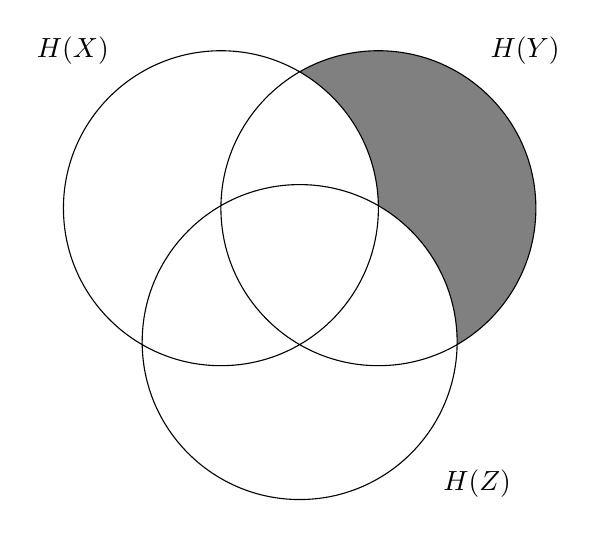
\begin{tikzpicture}
\scope
\clip \rectB
      \circleA;
\clip \rectB
      \circleC;
\fill[gray] \circleB;
\endscope
% outline:
\draw \circleA
      \circleB
      \circleC;
% labels:
\labelA{$H(X)$};
\labelB{$H(Y)$};
\labelC{$H(Z)$};     
\end{tikzpicture}
\end{center}
or using the predefined commands \texttt{filla}, \texttt{fillb}, etc. Specifying a colour is required, specifying a fill opacity between 0 and 1 is optional (default = 1):
\begin{center}
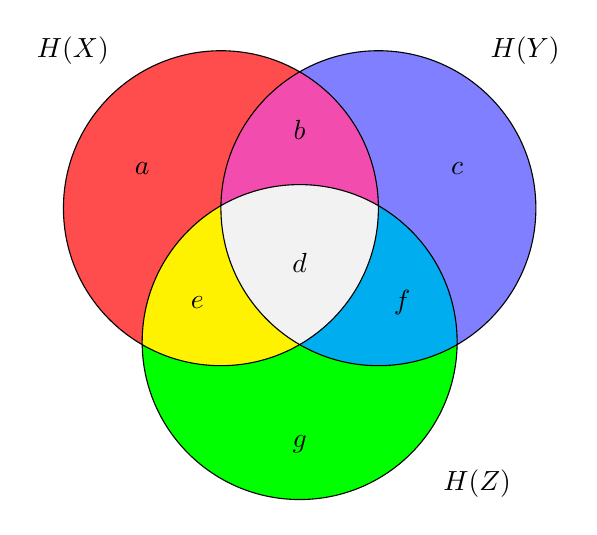
\begin{tikzpicture}
\filla[0.7]{red}
\fillb[0.7]{magenta}
\fillc[0.5]{blue}
\filld[0.1]{gray}
\fille{yellow}
\fillf{cyan}
\fillg{green}
% outline:
\draw \circleA
      \circleB
      \circleC;
% labels:
\labelA{$H(X)$};
\labelB{$H(Y)$};
\labelC{$H(Z)$};
% more labels:
\draw (-1,0.5) node {$a$}
      (1,1) node {$b$}
      (3,0.5) node {$c$}
      (1,-0.7) node {$d$}
      (-0.3,-1.2) node {$e$}
      (2.3,-1.2) node {$f$}
      (1,-3) node {$g$};
\end{tikzpicture}
\end{center}
\end{document}